\chapter{Introduction}
% \label{sec:chapter1}

%
The last decade has experienced a rapid growth in the world population, and, in the following years, it is expected the number of people to increase with a rate of $1.1\%$ for year, reaching $9.7$ billions in 2050 \cite{wpp}. As the world population increases, so the energy demand does. The increasing population and the limited ability to supply non-renewable energy, has led to a rise of power demand, especially in developing countries. This high energy demand has required an intensive usage of fossil energy, causing environmental pollution and changes in the climate.\\ 
Indeed, the increasing global temperature and the worsening of the air quality are posing a real problem for the environment. In the last years, some changes have been observed in Earth’s climate, primarily driven by human activities, particularly fossil fuel burning. \\

The biggest disadvantage of fossil fuels is that during the process of combustion in addition to produce energy, greenhouse gases (\gls{GHG}) are emitted \cite{greenhousegasemissions}. \\
These gases form a cope in the atmosphere, like glass in greenhouses, that traps the heat, increasing the earth's temperature. \\
For around a century, humans have relied on fossil fuels, like oil, natural gas and coil for everyday tasks: heating, transportation, to produce electricity. For this reason, the \gls{GHG} emission have reached historical peaks and are expected to increase in the following years \cite{co2predic}: in the year 2020, the concentration of \gls{CarbonDiox} in the atmosphere had risen to $48\%$ above its pre-industrial level (before 1750). \\

In order to improve the situation, the 2015 Paris Agreement set an ambition to limit global warming to well below $\SI{2}{\degreeCelsius}$ above pre-industrial levels and pursue efforts to limit it to $\SI{1.5}{\degreeCelsius}$ - in part by pursuing net carbon neutrality by 2050. The substantial reduction of global greenhouse gas emissions (including \gls{CarbonDiox})  will limit the increase of global temperature \cite{french_conference}. \\
Countries were asked to go through a process of decarbonization: the reduction of carbon dioxide emissions through the use of low carbon power sources. \\
%Renewable energy production has low or no waste products such as \gls{CarbonDiox} or other chemical pollutants.  \\
% These low carbon power sources usually are renewable energies such as sun, wind, geothermal heat and other natural sources.
These sources convert the energy coming through naturals elements (sun, wind, geothermal heat) in another form of energy, electricity for example, with low or no waste products such as \gls{CarbonDiox} or other chemical pollutants. 

\begin{figure}[H]
\centering
    % 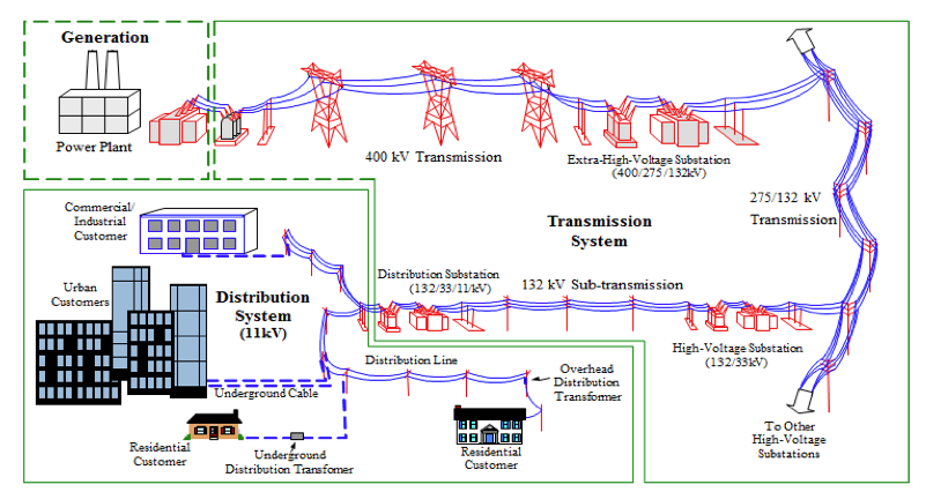
\includegraphics[width=.9\linewidth]{images/DN/HighMediumLowV.png}
    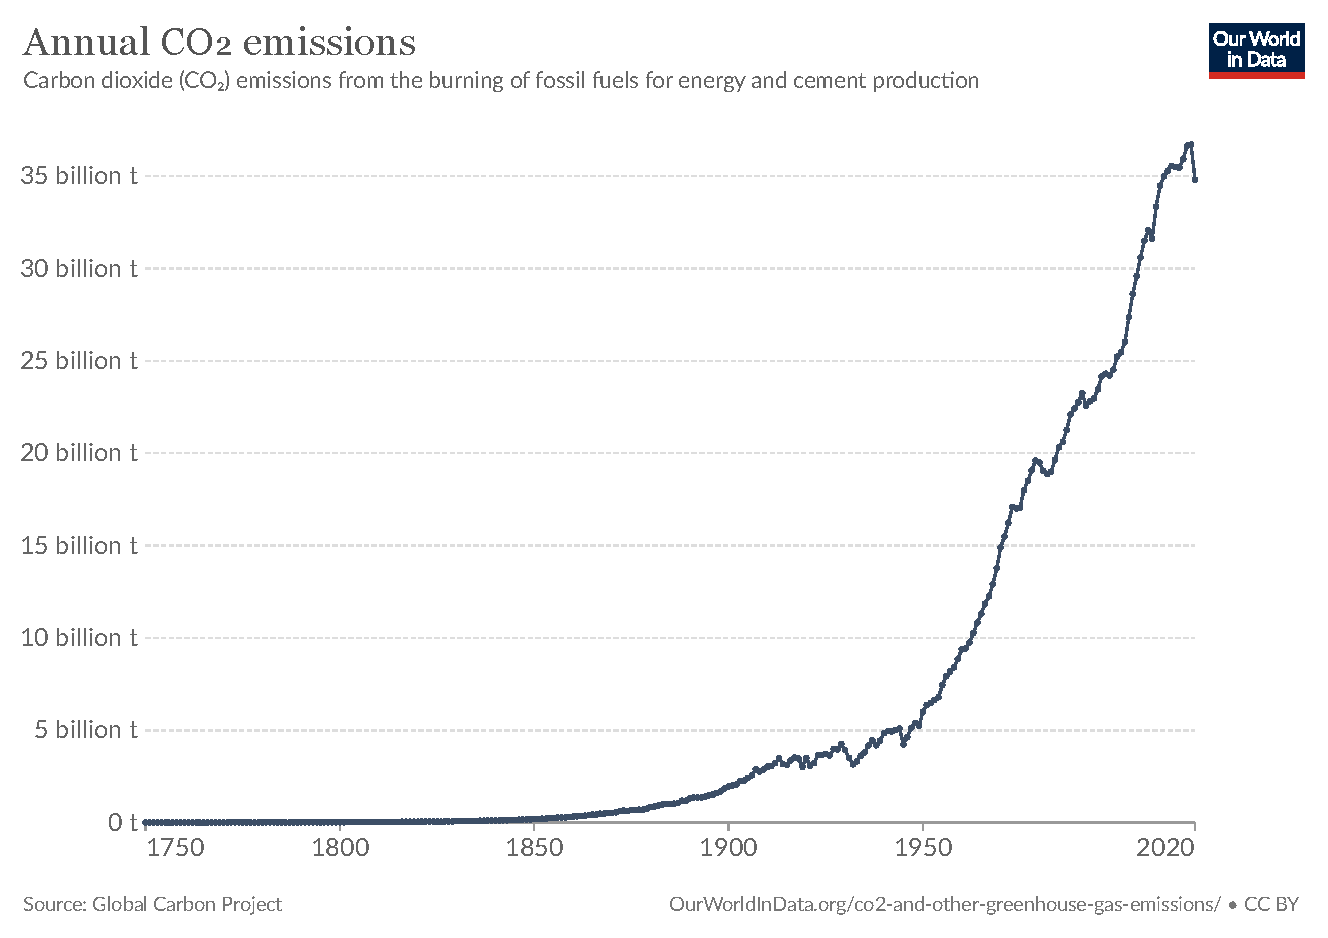
\includegraphics[width=.6\linewidth]{images/Introduction/annual-co2-emissions-per-country.pdf}
\caption[\gls{CarbonDiox} production over the years]{World \gls{CarbonDiox} production over the years \cite{C02prod}}
\end{figure}

Thanks to this emerging trend of decarbonization, more and more renewable power energy devices are introduced in the distribution networks \cite{owidenergy}. With the advantages of inexhaustibility and low impact on the environment, the high penetration of these renewables devices bring in some technical complications for the distribution of power and voltage in the grids. \\
The networks, that have been designed around the conventional centralized energy production, have to adapt to the new generators in the system. It is possible to say that the distribution networks are moving from unidirectional power flow (from the distribution system to the consumers) to a bidirectional power flow (in this case the consumers are also producers and the exceed energy can be transported from the consumers to the distribution system. They are also known as prosumers \cite{prosumers}). This switch from unidirectional to bidirectional power flow requires a smarter system that can handle in an efficient way the generation and distribution of voltage.\\

In the literature, this smarter way to control a distribution system is known as active network management (\gls{ANM}) and it refers to the design of control schemes that modulate the generators, the loads, and the distributed energy storages (\glspl{DES}), as well as other elements like switches, connected to the grid. \\


\section{Aim of the thesis}
\label{sec:aimthesis}
The aim of this thesis is to exploit data-driven approaches to forecast the future nodes' voltage based on historical measurements in a medium-voltage distribution system using machine learning techniques, in particular deep learning models. Predicting voltage fluctuation problems in the network would allow avoiding possible consequences related to these issues. Moreover, some control voltage techniques will be employed to avoid the network's critical situations, like for example over voltages problems.

% \section{Research methods}

\section{Thesis outline}
% Chapter 2 provides
% \\
% Chapter 3 ...

